\subsection{Variable dutycycle}

\subsubsection{ISense}
\textcolor{gray}{Meet \( V_{\text{osc}} \) en \(V_{out}\). Wat is de maximale duty cycle?}

Zonder \(I_{sense}\) aan te sluiten hebben we een duty cycle van ongeveer 99\% welke wordt gegeven door de waarde van \(C_T\).

\paragraph{NPN}
In \autoref{fig:Scopebeeld_NPN_1} is te zien dat de duty cycle bijna 100\% is. Met de maximale en minimale waarden aangegeven in \autoref{tab:npn_waarden2}. Maar ook te zien in deze tabel is dat de spanning over \(V_{Isense}\) met 0.7V daalt door de spanningsval over \(V_{be}\). Daarom voegen we een pnp transistor toe die de \(V_{osc}\) buffert. Dit wordt uitgewerkt in \autoref{par:pnp_npn_samen}.
 
\begin{figure}[b]
    \centering
    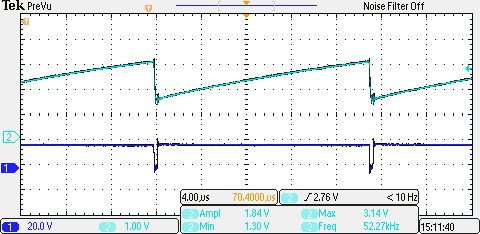
\includegraphics[width=0.7\linewidth]{img/hfd3/TEK00016.PNG}
    \caption{Scopebeeld van \(V_{osc}\) (licht blauw) en \(V_{Isense}\) (donker blauw)}
    \label{fig:Scopebeeld_NPN_1}
\end{figure}


\begin{figure}[b]
    \centering
    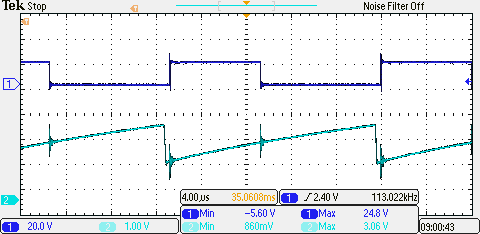
\includegraphics[width=0.7\linewidth]{img/hfd3/TEK00048.PNG}
    \caption{Scopebeeld van \(V_{out}\) (licht blauw) en \(V_{osc}\) (donker blauw)}
    \label{fig:scopebeeld_pnp_2}
\end{figure}


\begin{table}[h!]
\centering
\begin{tabular}{|l|c|}
\hline
\textbf{Parameter} & \textbf{Waarde (V)} \\ \hline
Max Vosc & 3,09 \\ \hline
Min Vosc & 1,43 \\ \hline
Max VIsense & 2,51 \\ \hline
Min VIsense & 0,89 \\ \hline
\end{tabular}
\caption{Gemeten spanningen bij alleen NPN-transistor}
\label{tab:npn_waarden2}
\end{table}


\paragraph{PNP}
\label{par:pnp_npn_samen}
Een PNP transistor wordt toegevoegd om \(V_{osc}\) te bufferen en door de spanningsval over \(V_{be}\) gaat de spanning over \(V_{osc}\) met 0.7V omhoog. Dit is te zien in \autoref{tab:pnp_npn_waarden}, ook in \autoref{fig:scopebeeld_pnp_2} zien we de dubbele buffer.

\begin{table}[h!]
\centering
\begin{tabular}{|l|c|}
\hline
\textbf{Parameter} & \textbf{Vosc (V)} \\ \hline
Max VIsense & 3,16 \\ \hline
Min VIsense & 1,4 \\ \hline
\end{tabular}
\caption{Gemeten spanningen bij PNP en NPN-transistor}
\label{tab:pnp_npn_waarden}
\end{table}
